\documentclass[russian, utf8, pointsubsection, emptystyle, simple]{eskdtext}
\usepackage[T2A]{fontenc}
\usepackage{eskdtotal}
\usepackage[math]{pscyr}
\usepackage{amssymb, amsmath, amsfonts, latexsym, amstext}
\usepackage{url}
\usepackage{multirow}
\usepackage{rotating}
\usepackage{ulem}
\usepackage{setspace}
\usepackage{graphicx}
\usepackage{longtable}
\usepackage{pdflscape}
\usepackage{itemsep}
\noitemsep
%\ESKDsectStyle{section}{\Large\bfseries}
\graphicspath{{pictures/}}

\usepackage{geometry}
\geometry{top=2cm}
\geometry{bottom=3.5cm}
\geometry{left=3.0cm}
\geometry{right=2cm}
\geometry{footskip=1.5cm}
\usepackage{fancyhdr}
\pagestyle{fancy}
\fancyhf{}
\renewcommand{\headrulewidth}{0pt}
\fancyfoot[C]{\thepage}

\usepackage{listings}
\lstset{language=C++,
  frame = ltrb,
  framesep = 5pt,
  basicstyle = \small\ttfamily,
  keywordstyle = \bfseries, 
  extendedchars = \true,
  identifierstyle = \bfseries\itshape, 
  commentstyle = \itshape,
  % stringstyle = \itshape, 
  numbers = left, 
  numberstyle = \scriptsize,
  breaklines = true,
  showspaces = true,
  showstringspaces = true
}
\renewcommand{\lstlistingname}{Листинг}

\ESKDtitle{Проектирование защиты программного обеспечения}
\ESKDdocName{Курсовая работа}
\ESKDsignature{ПГУ~3.090106.001}
\ESKDauthor{Захаров~М.\,А.}
\ESKDchecker{Фатеев~А\,.Г.}
\ESKDnormContr{Фатеев~А\,.Г.}
\ESKDcolumnIX{Гр.~06ПТ1}
\addto\captionsrussian{\def\refname{Список использованных источников}}

\usepackage[unicode]{hyperref}
\hypersetup{pdfkeywords = ПАСОИБ Фатеев,
colorlinks=true,
linkcolor=red,
citecolor=green,
urlcolor=cyan}

\begin{document}
\ESKDthisStyle{empty}
\newpage
\begin{center}
  \begin{singlespace}
    Министерство образования и науки РФ  \\
    Государственное образовательное учреждение высшего профессионального образования \\
    \vspace{0.25cm}
    <<ПЕНЗЕНСКИЙ ГОСУДАРСТВЕННЫЙ УНИВЕРСИТЕТ>> \\
    \medskip 
    \hrule height 1pt
    \vskip 1pt 
    \hrule
    \vskip 3pt
    Кафедра <<Информационная безопасность систем и технологий>>
  \end{singlespace}

  \vspace{8em}

  \textsc{\textbf{ПРОЕКТИРОВАНИЕ ЗАЩИТЫ ПРОГРАММНОГО ОБЕСПЕЧЕНИЯ}}\\[0.5cm]

  Пояснительная записка к курсовому проекту \\
  по дисциплине <<Программно-аппаратные средства обеспечения информационной безопасности>>\\[0.5cm]

  ПГУ 2.090106.001 ПЗ

  \vspace{8em}

  \begin{tabular}[h]{p{7cm}l}
    Руководитель КР,  & \\
    доцент, к.т.н. & \underline{\hspace{3cm}}Фатеев~А.\,Г.\\
    Исполнитель КР,  & \\
    студент & \underline{\hspace{3cm}}Захаров~М.\,А.
  \end{tabular}

  \vspace{\fill}

  Пенза 2011

\end{center}
\newpage

\begin{center}
  \Large{\textbf{РЕФЕРАТ}}
\end{center}

Отчёт \ESKDtotal{page}~с., 9~рис., \ESKDtotal{bibitem}~источника,
2~прил.

ЗАЩИТА ПРОГРАММНОГО ОБЕСПЕЧЕНИЯ, НЕСАНКЦИОНИРОВАННОЕ ИСПОЛЬЗОВАНИЕ,
ОТЛАДЧИК, ДИЗ\-АС\-СЕМБ\-ЛЕР, УТИЛИТА МОНИТОРИНГА, ХЭШ-ФУНКЦИЯ

Объектом исследования являются методы защиты программного обеспечения
от несанкционированного копирования.

Цель работы~--- разработка программной защиты приложения от
несанкционированного копирования.

В процессе работы были изучены сведения о защите программ от
несанкционированного копирования и методах ограничения
функциональности.

В результате исследования была разработана защита программы,
генерирующей псевдослучайную последовательность заданной длины, с
защитой от несанкционированного копирования методом ограничения
времени работы незарегистрированной программы. \newpage

%%% Local Variables: 
%%% mode: latex
%%% TeX-master: "../TermWork_OPOIB"
%%% End: 

\tableofcontents
\newpage
\hfill\parbox{6.5cm}{<<Утверждаю>>\\
  Зав. кафедрой ИБСТ\\
  \hbox to 6.5cm{\hrulefill С.\,Л.\,Зефиров}\\
  \def\hrf#1{\hbox to#1{\hrulefill}}
  <<\hrf{2em}>> \hrf{6em} \the\year~г.}	
	
\begin{center}\textbf{\normalfont\bfseries\large ЗАДАНИЕ}\\\textbf{на
    курсовую работу}\end{center}

\newpage

%%% Local Variables: 
%%% mode: latex
%%% TeX-master: "../TermWork_OPOIB"
%%% End: 

\newpage

\begin{center}
  \Large{\textbf{ВВЕДЕНИЕ}}
\end{center}
\addcontentsline{toc}{section}{Введение}

Целью данного курсового проектирования является разработка программной
защиты приложения от несанкционированного копирования.

Защита интеллектуальных ресурсов от незаконного использования является
на сегодняшний день одним из основных направлений разработки
программного обеспечения. Не существует абсолютно надежных методов
защиты. Можно утверждать, что достаточно квалифицированные системные
программисты, пользующиеся современными средствами анализа работы
программного обеспечения (отладчики, дизассемблеры, перехватчики
прерываний и т. д.), располагающие достаточным временем, смогут
преодолеть практически любую защиту. Поэтому при проектировании
системы защиты следует исходить из предположения, что рано или поздно
эта защита окажется снятой~\cite{1}. Целью проектирования должен быть выбор
такого способа защиты, который обеспечит невозможность
несанкционированного копирования для заранее определенного круга лиц и
в течение ограниченного времени.

В процессе выполнения курсового проекта производится разработка защиты
программы-генератора псевдослучайной последовательности от
несанкционированного копирования, за счет ограничения времени работы
программы. Разработанная защита должна быть исследована с целью
анализа стойкости.

\newpage

%%% Local Variables: 
%%% mode: latex
%%% TeX-master: "../TermWork_PASIOB"
%%% End: 


\section{Разработка и реализация алгоритма защиты}
\label{sec:--1}

\subsection{Описание целей и способа защиты}
\label{subsec:--1}

В соответствии с заданием на курсовой проект, защита программы от
несанкционированного копирования осуществляется посредством
ограничения времени работы незарегистрированной программы. Данный
способ защиты обеспечивает возможность ознакомления пользователя с
программой без ее приобретения. Это позволяет предоставить
использование программы пользователям, которые не планируют ее
постоянно использовать, либо хотят принять решение о
целесообразности ее приобретения. Для снятия ограничения по
использованию программы следует произвести регистрацию программы с
помощью пароля. Знание пароля является свидетельством прав на
обладание программой и должно предоставляться правообладателем.

Защита программы должна контролировать наличие регистрации. При этом
программа должна регистрироваться однажды и не требовать ввода пароля
при каждом запуске.  В качестве механизма определения возможностей
пользователя при работе с программой выступает признак регистрации
программы, сохраняемый в реестре операционной системы. В качестве
признака выступает текстовая строка, содержащая ключевую фразу.

Признак регистрации проверяется при запуске. В случае отсутствия
регистрации проверяется срок использования незарегистрированной
программы. Если он не превышает установленного, программа запускается,
в противном случае предлагается зарегистрировать программу. До
регистрации программы доступ к полезным функциям программы
блокируется.

При регистрации создается соответствующий ключ реестра, в который
записывается строка регистрации.

Пароль защищается в коде программы регистрации применением встроенной
в Visual Studio хэш-функции.

\subsection{Описание алгоритма защиты}
\label{subsec:--2}

При запуске программы проверяется наличие записи в ключе реестра. Если
ключ не найден, либо его содержимое не совпадает с признаком
регистрации, то осуществляется проверка срока использования
программы. Для этого из файла считывается дата установки программы. К
полученной дате прибавляется срок использования незарегистрированной
программы, равный 5 дням. Полученная дата сравнивается с текущей. Если
рассчитанная дата меньше текущей, доступ к полезным функциям программы
блокируется и пользователю предлагается произвести регистрацию
посредством пароля.

Если пользователь желает пройти регистрацию, то запускается процедура
регистрации. Процедура регистрации включает правильность проверки
пароля пользователя. Если пароль верен, в ключ реестра записывается
строка-признак регистрации. При вводе неверного пароля выдается
соответствующее сообщение, и регистрация не проходит.  Если содержание
ключа реестра, используемого программой, соответствует установленному
признаку регистрации, то программа считается зарегистрированной и
запускается без проверки срока использования.

Блок-схема разработанного алгоритма приведена в
Приложении~А.

\subsection{Описание программной реализации алгоритма защиты}
\label{sec:--3}

Для реализации разработанного алгоритма защиты программы была
разработана программа, выполняющая генерацию псевдослучайной
последовательности со встроенной защитой от несанкционированного
копирования, а также программа установки, осуществляющая настройку
параметров защиты для основной программы. 

Для разработки программы использовалась интегрированная среда
разработки Visual Studio Express 2010. Для написания программы был
использован язык программирования Visual C++.  Функция регистрации
позволяет снять ограничения для легальных пользователей. Она включает
проверку пароля пользователя и, в случае ввода правильного пароля,
создает ключ реестра, содержащий признак регистрации. Данная функция
реализована в виде обработчика нажатия кнопки на главной форме
проекта (листинг~\ref{1.cpp}).

\begin{lstlisting}[caption = {Функция регистрации}, label = {1.cpp}]
private: System::Void button2_Click(System::Object^  sender, System::EventArgs^  e) {
 int pass = this->textBox1->Text->GetHashCode();
 int right_pass = 1364505728; 
 if(pass==right_pass)
 {
	  RegistryKey^ rk = nullptr;
	  rk = Registry::CurrentUser->OpenSubKey("GPSP",true);
	  if (rk==nullptr)
	  {
			 RegistryKey^ rk = Registry::CurrentUser->CreateSubKey("GPSP");
			 rk->SetValue("line","forza");
			 rk->Close();
	  }					
	  else
	  {
			 Registry::CurrentUser->DeleteSubKey("GPSP");
			 RegistryKey^ rk = Registry::CurrentUser->CreateSubKey("GPSP");
			 rk->SetValue("line","forza");
			 rk->Close();
	  }
	  this->groupBox1->Hide();
	  this->groupBox2->Show();
	  MessageBox::Show("Зарегистрировано");
 }
 else
 {
	 MessageBox::Show("Неправильный пароль");
 }

} 
\end{lstlisting}

Основная программа содержит функцию проверки наличия ключа реестра и
правильность значения, записанного в него. 

Данная функция вызывается при загрузке программы, при обработке
события \texttt{Form\_Load}. Если регистрация отсутствует, программа
проверяет, не превышен ли срок использования программы. Для этого из
файла созданного при установке программы считывается дата
установки. Сравнение дат, осуществляется с использованием методов
встроенного класса \texttt{DateTime} (листинг~\ref{2.cpp})~\cite{2}.

\begin{lstlisting}[caption = {Проверка признака регистрации}, label = {2.cpp}]
 bool reg = true;
 RegistryKey^ rk = nullptr;
 rk = Registry::CurrentUser->OpenSubKey("GPSP",true);
 if (rk==nullptr)
 {
	reg = false;
 }
 else
 {
	 String^ value = rk->GetValue("line")->ToString();
	 if(value!="forza") reg = false; 
 }
 DateTime^ dt = DateTime::Now;
 if(!reg)
 {
	 
	 StreamReader^ read_date = gcnew StreamReader("param");
	 DateTime^ start = Convert::ToDateTime(read_date->ReadLine()); 
	 if(DateTime::Compare(start->AddDays(5), dt->Date)<0)
	 {
		 MessageBox::Show("Срок использования незарегистрированной версии истек. Хотите зарегистрировать программу");
		 this->groupBox2->Hide();
	 }
	 else this->groupBox1->Hide();
 }
 else this->groupBox1->Hide(); 
\end{lstlisting}

Интерфейс основной полезной программы приведен на рисунке~\ref{fig:1}.

\begin{figure}[h!]
  \centering
  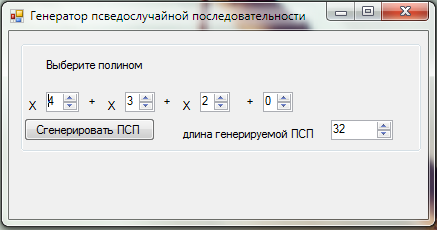
\includegraphics[]{interface}
  \caption{Интерфейс программы}
  \label{fig:1}
\end{figure}

Для проверки корректности работы защиты программы было осуществлено
изменение системной даты на 7 дней вперед. На рисунке~\ref{fig:2}
отображено сообщение об окончании периода использования
незарегистрированной программы.

\begin{figure}[h!]
  \centering
  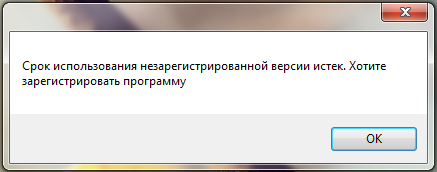
\includegraphics[]{register_message}
  \caption{Сообщение об окончании периода использования
    незарегистрированной программы}
  \label{fig:2}
\end{figure}

Блокирование полезных функций программы после окончания периода
использования незарегистрированной программы представлено на
рисунке~\ref{fig:3}.

\begin{figure}[h!]
  \centering
  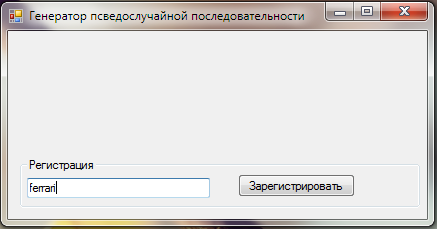
\includegraphics[]{register}
  \caption{Блокирование полезных функций после окончания периода
    использования незарегистрированной программы}
  \label{fig:3}
\end{figure}

Полный текст основной программы, а также программы установки приведен
в Приложении Б.

\section{Анализ стойкости использованного алгоритма защиты}
\label{sec:--4}

В ходе исследования выявляются сведения, которые могут быть
использованы нарушителем для проведения атак на защиту программы. На
данном этапе использовались следующие программные средства
анализа\cite{4}:

\vspace{-5mm}
\begin{itemize}
\item дизассемблер \textit{IDA}, позволяющий произвести статическое
  исследование дизассемблированного листинга программы;
\item утилита мониторинга \textit{ProcessMonitor}, осуществляющая
  контроль активности приложения при обращениях к ресурсам файловой
  системы, реестра и системным вызовам;
\item отладчик \textit{OllyDbg}, позволяющий произвести динамическое
  исследование логики работы программы.
\end{itemize}

\subsection{Анализ защиты с использованием дизассемблера}
\label{sec:--5}

Первым этапом исследования являлось дизассемблирование программы. В
результате анализа полученного кода выявлен механизм проверки
регистрации, представленный на рисунке~\ref{fig:4}.

\begin{figure}[h!]
  \centering
  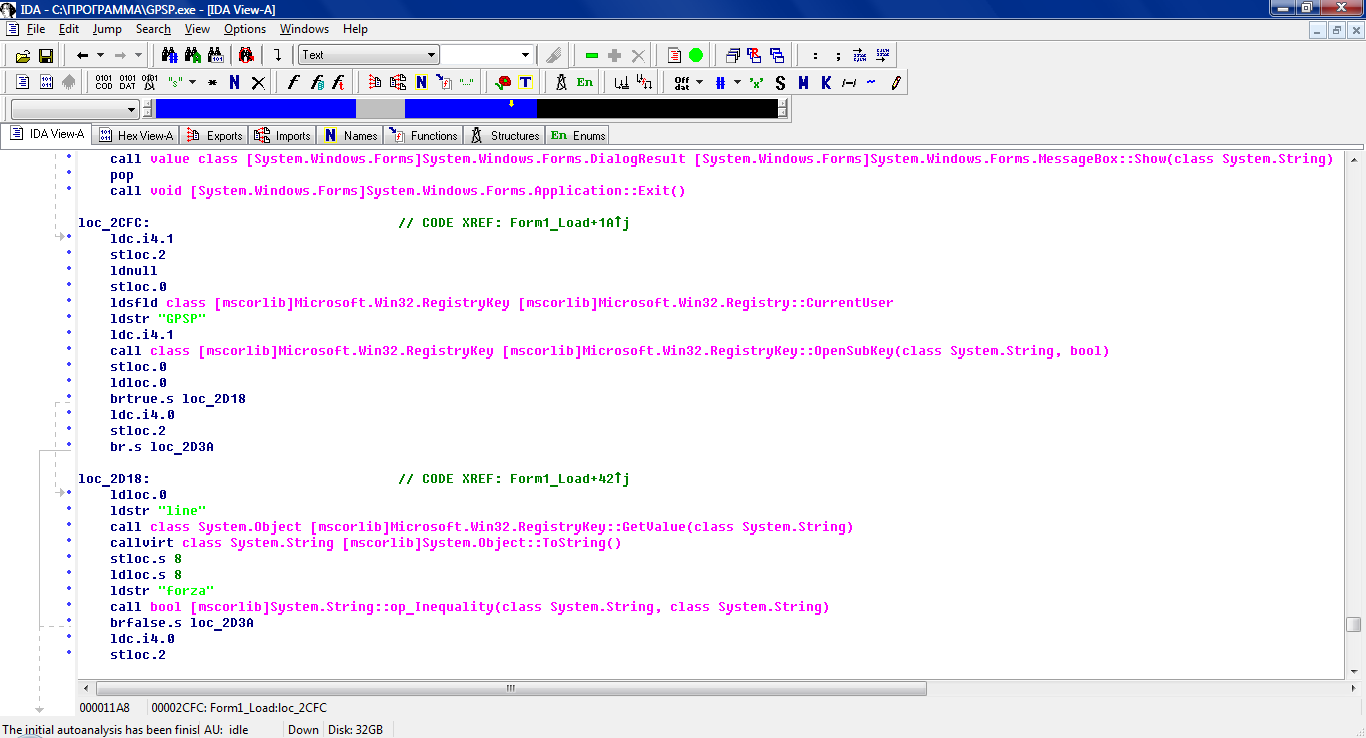
\includegraphics[width=\textwidth]{register_chech}
  \caption{Функция проверки регистрации программы}
  \label{fig:4}
\end{figure}

На данном рисунке отмечены функции считывания значения ключа реестра и
функция сравнения с признаком регистрации. Признак регистрации при
этом хранится в явном виде (строка). Данные сведения могут быть
использованы при создании признака регистрации несанкционированным
способом.

В обработчике кнопки регистрации были выявлены механизмы проверки
пароля пользователя и хэш от верного пароля, а также создания признака
регистрации в ключе реестра. Данные элементы отмечены на
рисунке~\ref{fig:5}.

\begin{figure}[h!]
  \centering
  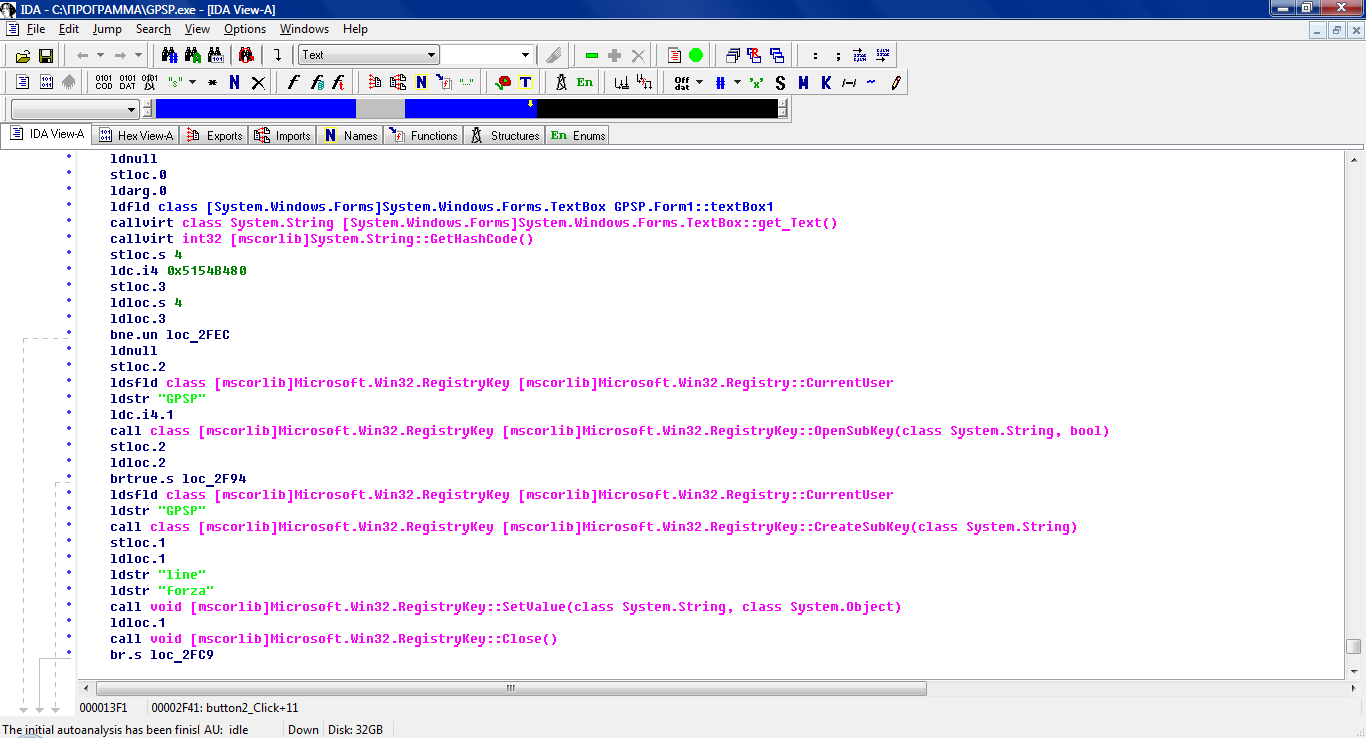
\includegraphics[width=\textwidth]{check_password}
  \caption{Проверка пароля пользователя при регистрации}
  \label{fig:5}
\end{figure}

Таким образом, атака на пароль затруднена, поскольку в программе
хранится лишь проверочное значение хэш, и наиболее эффективным
способом будет простой перебор всех возможных паролей.  

Также была исследована функция проверки срока использования
программы. Данная функция представлена на рисунке~\ref{fig:6}.

\begin{figure}[h!]
  \centering
  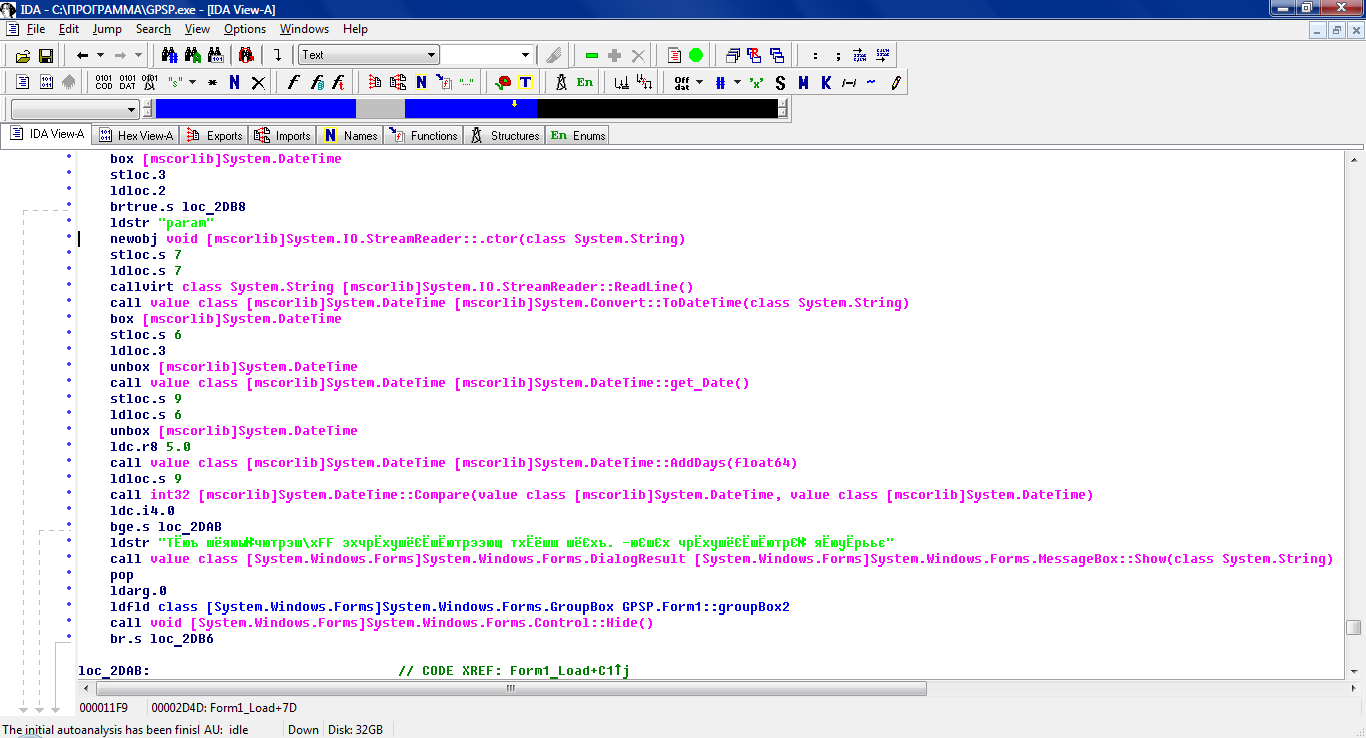
\includegraphics[width=\textwidth]{check_date}
  \caption{Функция проверки срока использования программы}
  \label{fig:6}
\end{figure}

На рисунке~\ref{fig:6} отмечено считывание даты установки из файла
\texttt{param}, а также срок равный 5 дням и функция сравнения
дат. Данные сведения могут быть использованы при попытках модификации
даты установки, либо при модификации программы.

\subsection{Анализ защиты с использованием монитора процессов}

Далее была проанализированы обращения программы к ресурсам файловой
системы и реестра при запуске и проверке регистрации, с помощью
программы \textit{ProcessMonitor}. На рисунке~\ref{fig:7} представлено
считывание признака регистрации из ключа реестра при запуске.

\begin{figure}[h!]
  \centering
  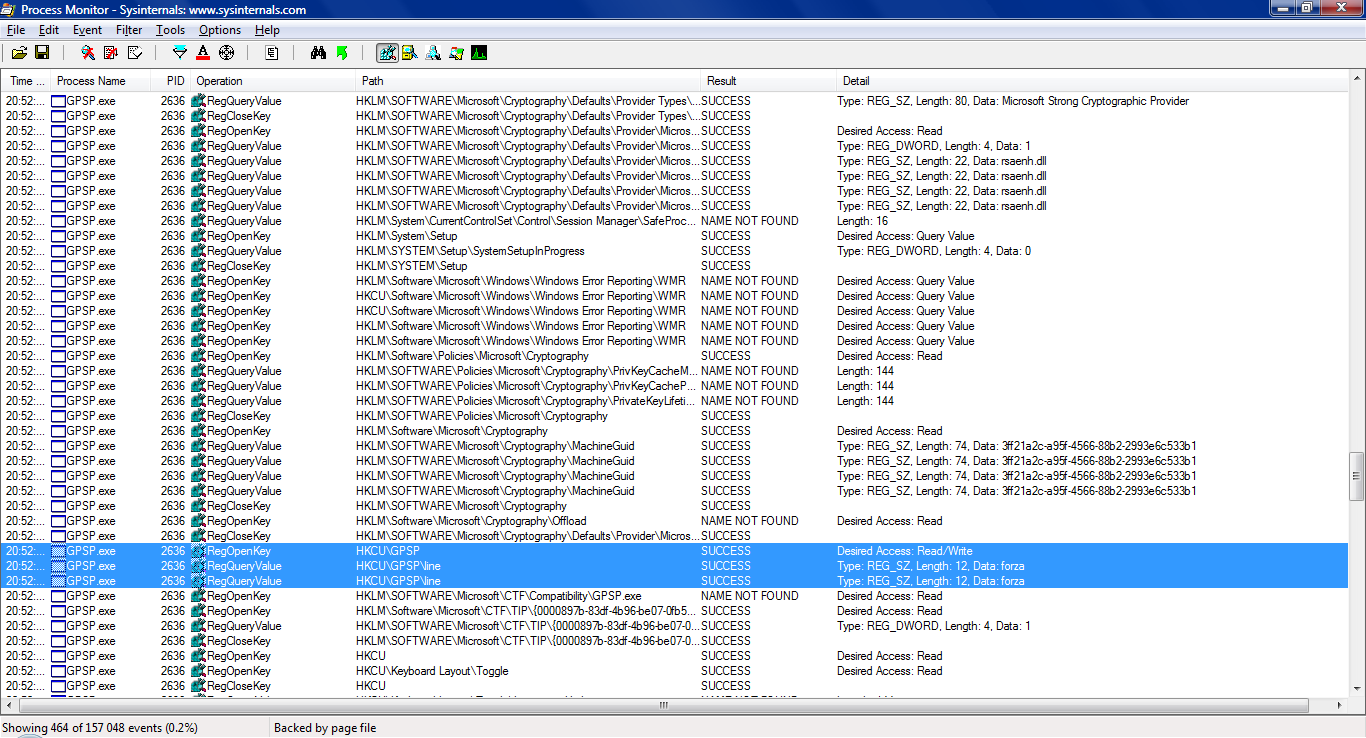
\includegraphics[width=\textwidth]{process}
  \caption{Обращения к реестру для проверки признака регистрации}
  \label{fig:7}
\end{figure}

Из полученных сведений можно построить алгоритм работы механизма
проверки регистрации. Кроме того, можно установить содержимое ключа
регистрации программы (строка-признак регистрации \texttt{forza}
отображается как содержимое ключа). Данные сведения могут быть
использованы при создании признака регистрации несанкционированным
способом.

\subsection{Анализ защиты с использованием отладчика}

В ходе исследования средствами отладчика выявлен условный переход,
управляющий проверкой регистрации. На рисунке~\ref{fig:8} на него
установлена точка останова.

\begin{figure}[h!]
  \centering
  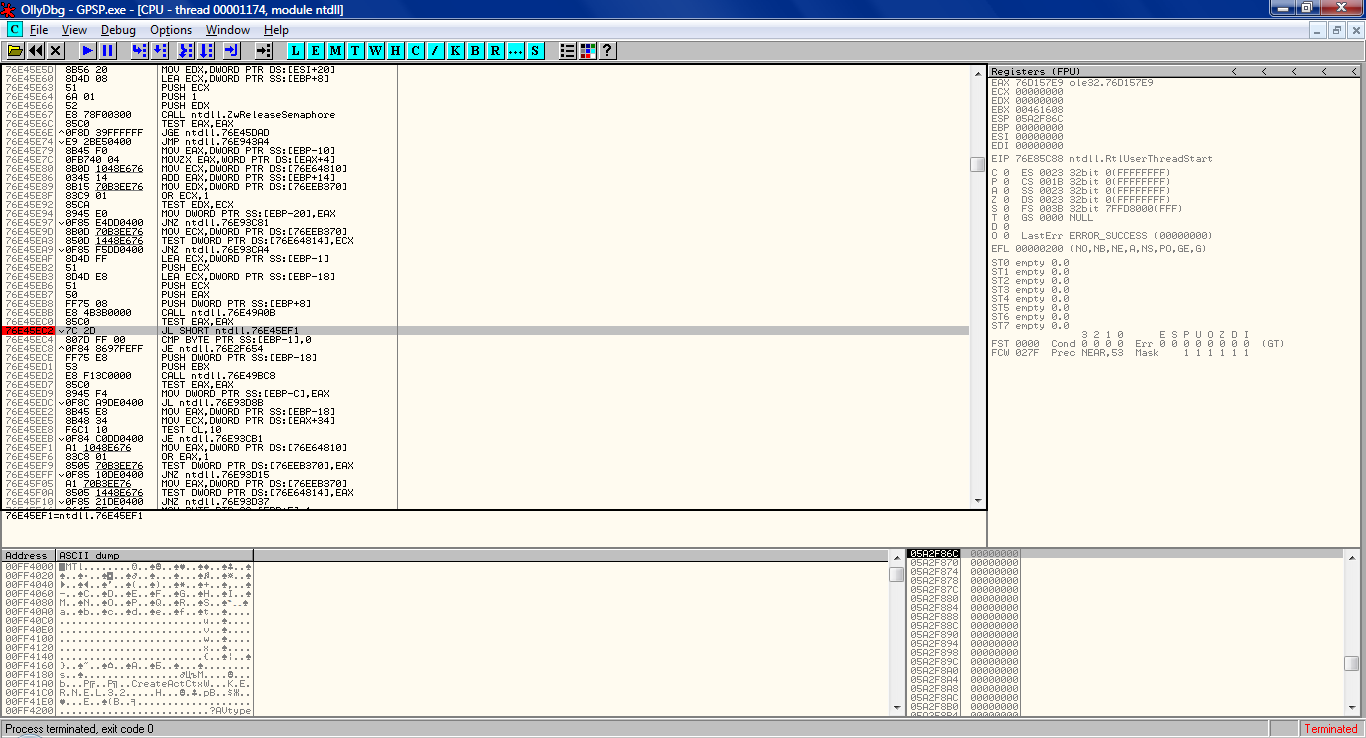
\includegraphics[width=\textwidth]{olly}
  \caption{Условный переход, управляющий проверкой регистрации}
  \label{fig:8}
\end{figure}

Модификация данного условного перехода средствами отладчика (например,
отключение проверки заменой перехода на команду NOP) приведет к снятию
защиты программы (результаты проверки не будут обрабатываться для
управления загрузкой программы).

В ходе исследования были выявлены уязвимости, позволяющие обойти
защиту программы: возможность изучения механизмов регистрации и
проверки регистрации, незащищенное хранение признака регистрации,
возможность модификации программы с целью отключения защиты.

Для повышения защиты программы следует ввести следующие усиления~\cite{4}:
\vspace{-5mm}
\begin{itemize}
\item разделение признака регистрации на несколько файлов и их
  шифрование с использованием данных даты установки, для вычисления
  ключа;
\item использование самомодифицирующегося кода: шифрование \linebreak
  критических участков программы и расшифровка их
  непосредственно в память процесса;
\item использование средств защиты от отладки;
\item защита файла, хранящего дату установки с использованием
  шифрования;
\item усложнения алгоритма работы программы с помощью ложных ветвей
  алгоритма и функций, не влияющих на работу программы;
\item отказ от использования осмысленных имен функций и использование
  функций переходников.
\end{itemize}

\cleardoublepage


%%% Local Variables: 
%%% mode: latex
%%% TeX-master: "../TermWork_PASIOB"
%%% End: 

\newpage
\begin{center}
  \Large{\textbf{ЗАКЛЮЧЕНИЕ}}
\end{center}
\addcontentsline{toc}{section}{Заключение}

В процессе выполнения курсового проекта были изучены сведения о защите
программ от несанкционированного копирования и методах ограничения
функциональности.  В результате выполнения курсового проекта
разработана защита программы, генерирующей псевдослучайную
последовательность заданной длины, с защитой от несанкционированного
копирования методом ограничения времени работы незарегистрированной
программы.

Для разработанной защиты был проведен анализ стойкости и сформированы
предложения по устранению выявленных недостатков.

Таким образом, требования, описанные в техническом задании на данный
курсовой проект, были выполнены полностью.

\newpage


\begin{thebibliography}{99}
\bibitem{1} Александр Фролов, Григорий Фролов. MS-DOS для
  программиста~М.: Диалог-МИФИ, 1995, 253 стр.
\bibitem{2} Самоучитель хакера: Подробное иллюстрированное
  руководство: Alex Atsctoy.~--- М.: «Лучшие книги», 2005.~--- 192 с.
\bibitem{3} Взлом программного обеспечения: анализ и использование
  кода: Перевод с английского~--- М.: Издательский дом «Вильямc»,
  2005.~--- 400 с.
\bibitem{4} Защита от взлома: Пер. с англ. Слинкина А. А.~--- М.:
  Издательский Дом ДМК-пресс, 2006.~--- 784 с.
\end{thebibliography}

\newpage{}

\begin{center}
  \Large{\textbf{ПРИЛОЖЕНИЕ А}}\\
  \normalsize (справочное) \\ \textbf{Алгоритм защиты программы}
\end{center}
\addcontentsline{toc}{section}{Приложение А Алгоритм защиты программы}
\label{AppendixA}

\begin{figure}[h!]
  \centering
  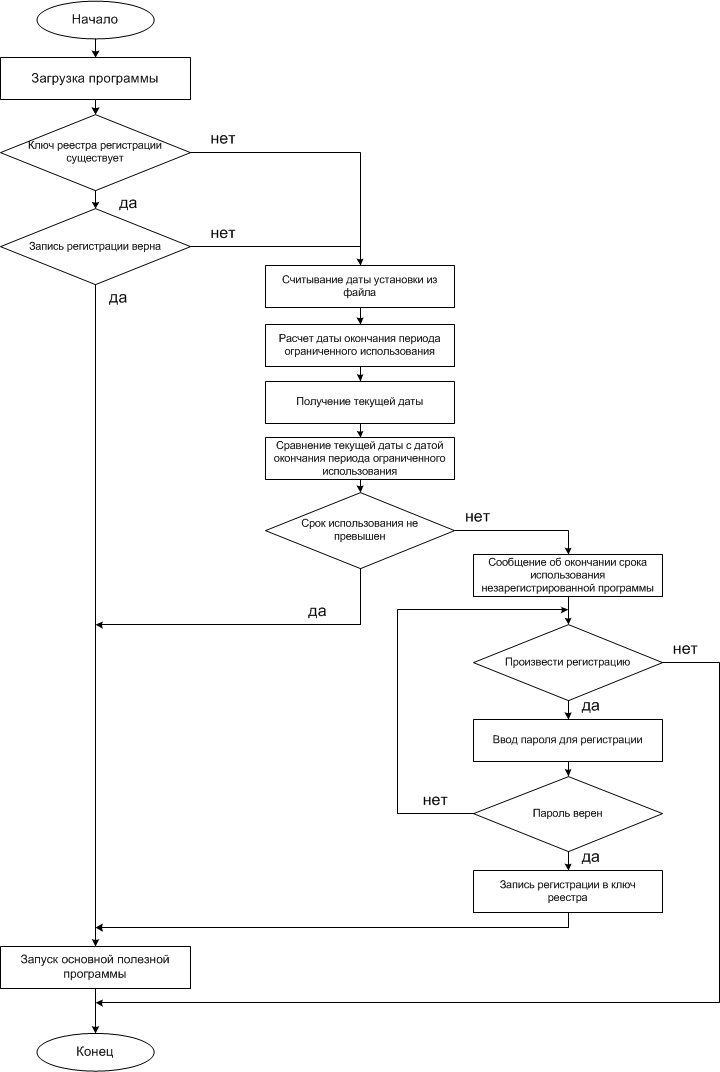
\includegraphics[height = 0.8 \textheight, keepaspectratio]{alg}
\end{figure}
\begin{center}
  Рисунок А.1 --- Алгоритм защиты программы
\end{center}

\newpage{}



%%% Local Variables: 
%%% mode: latex
%%% TeX-master: "../TermWork_PASIOB"
%%% End: 

\begin{center}
  \Large{\textbf{ПРИЛОЖЕНИЕ Б}}\\
  \normalsize (справочное) \\ \textbf{Листинги разработанных программ}
\end{center}
\addcontentsline{toc}{section}{Приложение Б Листинги разработанных программ}
\label{AppendixB}

\small

\begin{lstlisting}[caption = {ПРОГРАММА УСТАНОВКИ}, label = {4.cpp}]

#pragma once


namespace GPSP_install {

using namespace System;
using namespace System::ComponentModel;
using namespace System::Collections;
using namespace System::Windows::Forms;
using namespace System::Data;
using namespace System::Drawing;
using namespace System::IO;

/// <summary>
/// Сводка для Form1
///
/// Внимание! При изменении имени этого класса необходимо также изменить
///	     свойство имени файла ресурсов ("Resource File Name") для средства компиляции управляемого ресурса,
///	     связанного со всеми файлами с расширением .resx, от которых зависит данный класс. В противном случае,
///	     конструкторы не смогут правильно работать с локализованными
///	     ресурсами, сопоставленными данной форме.
/// </summary>
public ref class Form1 : public System::Windows::Forms::Form
{
public:
Form1(void)
{
	InitializeComponent();
	//
	//TODO: добавьте код конструктора
	//
}

protected:
/// <summary>
/// Освободить все используемые ресурсы.
/// </summary>
~Form1()
{
	if (components)
	{
		delete components;
	}
}
private: System::Windows::Forms::Button^  button1;
protected: 

private:
/// <summary>
/// Требуется переменная конструктора.
/// </summary>
System::ComponentModel::Container ^components;

#pragma region Windows Form Designer generated code
/// <summary>
/// Обязательный метод для поддержки конструктора - не изменяйте
/// содержимое данного метода при помощи редактора кода.
/// </summary>
void InitializeComponent(void)
{
	this->button1 = (gcnew System::Windows::Forms::Button());
	this->SuspendLayout();
	// 
	// button1
	// 
	this->button1->Location = System::Drawing::Point(12, 22);
	this->button1->Name = L"button1";
	this->button1->Size = System::Drawing::Size(75, 23);
	this->button1->TabIndex = 0;
	this->button1->Text = L"Установить";
	this->button1->UseVisualStyleBackColor = true;
	this->button1->Click += gcnew System::EventHandler(this, &Form1::button1_Click);
	// 
	// Form1
	// 
	this->AutoScaleDimensions = System::Drawing::SizeF(6, 13);
	this->AutoScaleMode = System::Windows::Forms::AutoScaleMode::Font;
	this->ClientSize = System::Drawing::Size(198, 58);
	this->Controls->Add(this->button1);
	this->Name = L"Form1";
	this->Text = L"Установка";
	this->ResumeLayout(false);

}
#pragma endregion
private: System::Void button1_Click(System::Object^  sender, System::EventArgs^	 e) {
	 FolderBrowserDialog^ folder_dialog = gcnew FolderBrowserDialog();
	 folder_dialog->ShowDialog();
	 if(folder_dialog->SelectedPath != "")
	 {
		 StreamWriter^ write = gcnew StreamWriter(folder_dialog->SelectedPath + "\\param");
		 DateTime^ dt = DateTime::Now;
		 write->WriteLine(dt->ToLongDateString());
		 write->Close();
		 File::Copy("GPSP.exe", folder_dialog->SelectedPath + "\\GPSP.exe");
		 MessageBox::Show("Установлено");
	 }
 }
};
}
\end{lstlisting}

\begin{lstlisting}[caption = {ОСНОВНАЯ ПОЛЕЗНАЯ ПРОГРАММА}, label = {4.cpp}]
#pragma once
namespace GPSP {

using namespace System;
using namespace System::ComponentModel;
using namespace System::Collections;
using namespace System::Windows::Forms;
using namespace System::Data;
using namespace System::Drawing;
using namespace System::IO;
using namespace Microsoft::Win32;

	

/// <summary>
/// Сводка для Form1
///
/// Внимание! При изменении имени этого класса необходимо также изменить
///	     свойство имени файла ресурсов ("Resource File Name") для средства компиляции управляемого ресурса,
///	     связанного со всеми файлами с расширением .resx, от которых зависит данный класс. В противном случае,
///	     конструкторы не смогут правильно работать с локализованными
///	     ресурсами, сопоставленными данной форме.
/// </summary>
public ref class Form1 : public System::Windows::Forms::Form
{
public:
	Form1(void)
	{
		InitializeComponent();
		//
		//TODO: добавьте код конструктора
		//
	}

protected:
	/// <summary>
	/// Освободить все используемые ресурсы.
	/// </summary>
	~Form1()
	{
		if (components)
		{
			delete components;
		}
	}
private: System::Windows::Forms::Label^	 label1;
protected: 
private: System::Windows::Forms::NumericUpDown^	 numericUpDown1;
private: System::Windows::Forms::Label^	 label2;
private: System::Windows::Forms::Label^	 label3;
private: System::Windows::Forms::NumericUpDown^	 numericUpDown2;
private: System::Windows::Forms::Label^	 label4;
private: System::Windows::Forms::Label^	 label5;
private: System::Windows::Forms::NumericUpDown^	 numericUpDown3;
private: System::Windows::Forms::Label^	 label6;
private: System::Windows::Forms::NumericUpDown^	 numericUpDown4;
private: System::Windows::Forms::Label^	 label8;
private: System::Windows::Forms::Button^  button1;
private: System::Windows::Forms::NumericUpDown^	 numericUpDown5;
private: System::Windows::Forms::Label^	 label7;
private: System::Windows::Forms::GroupBox^  groupBox1;
private: System::Windows::Forms::Button^  button2;
private: System::Windows::Forms::TextBox^  textBox1;
private: System::Windows::Forms::GroupBox^  groupBox2;

private:
	/// <summary>
	/// Требуется переменная конструктора.
	/// </summary>
	System::ComponentModel::Container ^components;

#pragma region Windows Form Designer generated code
/// <summary>
/// Обязательный метод для поддержки конструктора - не изменяйте
/// содержимое данного метода при помощи редактора кода.
/// </summary>
void InitializeComponent(void)
{
this->label1 = (gcnew System::Windows::Forms::Label());
this->numericUpDown1 = (gcnew System::Windows::Forms::NumericUpDown());
this->label2 = (gcnew System::Windows::Forms::Label());
this->label3 = (gcnew System::Windows::Forms::Label());
this->numericUpDown2 = (gcnew System::Windows::Forms::NumericUpDown());
this->label4 = (gcnew System::Windows::Forms::Label());
this->label5 = (gcnew System::Windows::Forms::Label());
this->numericUpDown3 = (gcnew System::Windows::Forms::NumericUpDown());
this->label6 = (gcnew System::Windows::Forms::Label());
this->numericUpDown4 = (gcnew System::Windows::Forms::NumericUpDown());
this->label8 = (gcnew System::Windows::Forms::Label());
this->button1 = (gcnew System::Windows::Forms::Button());
this->numericUpDown5 = (gcnew System::Windows::Forms::NumericUpDown());
this->label7 = (gcnew System::Windows::Forms::Label());
this->groupBox1 = (gcnew System::Windows::Forms::GroupBox());
this->button2 = (gcnew System::Windows::Forms::Button());
this->textBox1 = (gcnew System::Windows::Forms::TextBox());
this->groupBox2 = (gcnew System::Windows::Forms::GroupBox());
(cli::safe_cast<System::ComponentModel::ISupportInitialize^  >(this->numericUpDown1))->BeginInit();
(cli::safe_cast<System::ComponentModel::ISupportInitialize^  >(this->numericUpDown2))->BeginInit();
(cli::safe_cast<System::ComponentModel::ISupportInitialize^  >(this->numericUpDown3))->BeginInit();
(cli::safe_cast<System::ComponentModel::ISupportInitialize^  >(this->numericUpDown4))->BeginInit();
(cli::safe_cast<System::ComponentModel::ISupportInitialize^  >(this->numericUpDown5))->BeginInit();
this->groupBox1->SuspendLayout();
this->groupBox2->SuspendLayout();
this->SuspendLayout();
// 
// label1
// 
this->label1->AutoSize = true;
this->label1->Location = System::Drawing::Point(22, 20);
this->label1->Name = L"label1";
this->label1->Size = System::Drawing::Size(104, 13);
this->label1->TabIndex = 0;
this->label1->Text = L"Выберите полином";
// 
// numericUpDown1
// 
this->numericUpDown1->Location = System::Drawing::Point(25, 54);
this->numericUpDown1->Maximum = System::Decimal(gcnew cli::array< System::Int32 >(4) {31, 0, 0, 0});
this->numericUpDown1->Minimum = System::Decimal(gcnew cli::array< System::Int32 >(4) {4, 0, 0, 0});
this->numericUpDown1->Name = L"numericUpDown1";
this->numericUpDown1->Size = System::Drawing::Size(33, 20);
this->numericUpDown1->TabIndex = 1;
this->numericUpDown1->Value = System::Decimal(gcnew cli::array< System::Int32 >(4) {4, 0, 0, 0});
// 
// label2
// 
this->label2->AutoSize = true;
this->label2->Location = System::Drawing::Point(5, 61);
this->label2->Name = L"label2";
this->label2->Size = System::Drawing::Size(14, 13);
this->label2->TabIndex = 2;
this->label2->Text = L"Х";
// 
// label3
// 
this->label3->AutoSize = true;
this->label3->Location = System::Drawing::Point(65, 56);
this->label3->Name = L"label3";
this->label3->Size = System::Drawing::Size(13, 13);
this->label3->TabIndex = 3;
this->label3->Text = L"+";
// 
// numericUpDown2
// 
this->numericUpDown2->Location = System::Drawing::Point(104, 54);
this->numericUpDown2->Maximum = System::Decimal(gcnew cli::array< System::Int32 >(4) {31, 0, 0, 0});
this->numericUpDown2->Minimum = System::Decimal(gcnew cli::array< System::Int32 >(4) {3, 0, 0, 0});
this->numericUpDown2->Name = L"numericUpDown2";
this->numericUpDown2->Size = System::Drawing::Size(30, 20);
this->numericUpDown2->TabIndex = 4;
this->numericUpDown2->Value = System::Decimal(gcnew cli::array< System::Int32 >(4) {3, 0, 0, 0});
// 
// label4
// 
this->label4->AutoSize = true;
this->label4->Location = System::Drawing::Point(84, 61);
this->label4->Name = L"label4";
this->label4->Size = System::Drawing::Size(14, 13);
this->label4->TabIndex = 5;
this->label4->Text = L"Х";
// 
// label5
// 
this->label5->AutoSize = true;
this->label5->Location = System::Drawing::Point(159, 61);
this->label5->Name = L"label5";
this->label5->Size = System::Drawing::Size(14, 13);
this->label5->TabIndex = 8;
this->label5->Text = L"Х";
// 
// numericUpDown3
// 
this->numericUpDown3->Location = System::Drawing::Point(179, 54);
this->numericUpDown3->Maximum = System::Decimal(gcnew cli::array< System::Int32 >(4) {31, 0, 0, 0});
this->numericUpDown3->Minimum = System::Decimal(gcnew cli::array< System::Int32 >(4) {2, 0, 0, 0});
this->numericUpDown3->Name = L"numericUpDown3";
this->numericUpDown3->Size = System::Drawing::Size(30, 20);
this->numericUpDown3->TabIndex = 7;
this->numericUpDown3->Value = System::Decimal(gcnew cli::array< System::Int32 >(4) {2, 0, 0, 0});
// 
// label6
// 
this->label6->AutoSize = true;
this->label6->Location = System::Drawing::Point(140, 56);
this->label6->Name = L"label6";
this->label6->Size = System::Drawing::Size(13, 13);
this->label6->TabIndex = 6;
this->label6->Text = L"+";
// 
// numericUpDown4
// 
this->numericUpDown4->Location = System::Drawing::Point(242, 54);
this->numericUpDown4->Maximum = System::Decimal(gcnew cli::array< System::Int32 >(4) {1, 0, 0, 0});
this->numericUpDown4->Name = L"numericUpDown4";
this->numericUpDown4->Size = System::Drawing::Size(30, 20);
this->numericUpDown4->TabIndex = 10;
// 
// label8
// 
this->label8->AutoSize = true;
this->label8->Location = System::Drawing::Point(223, 56);
this->label8->Name = L"label8";
this->label8->Size = System::Drawing::Size(13, 13);
this->label8->TabIndex = 9;
this->label8->Text = L"+";
// 
// button1
// 
this->button1->Location = System::Drawing::Point(3, 80);
this->button1->Name = L"button1";
this->button1->Size = System::Drawing::Size(131, 23);
this->button1->TabIndex = 11;
this->button1->Text = L"Сгенерировать ПСП";
this->button1->UseVisualStyleBackColor = true;
this->button1->Click += gcnew System::EventHandler(this, &Form1::button1_Click);
// 
// numericUpDown5
// 
this->numericUpDown5->Location = System::Drawing::Point(310, 82);
this->numericUpDown5->Maximum = System::Decimal(gcnew cli::array< System::Int32 >(4) {1000, 0, 0, 0});
this->numericUpDown5->Minimum = System::Decimal(gcnew cli::array< System::Int32 >(4) {32, 0, 0, 0});
this->numericUpDown5->Name = L"numericUpDown5";
this->numericUpDown5->Size = System::Drawing::Size(62, 20);
this->numericUpDown5->TabIndex = 12;
this->numericUpDown5->Value = System::Decimal(gcnew cli::array< System::Int32 >(4) {32, 0, 0, 0});
// 
// label7
// 
this->label7->AutoSize = true;
this->label7->Location = System::Drawing::Point(159, 89);
this->label7->Name = L"label7";
this->label7->Size = System::Drawing::Size(138, 13);
this->label7->TabIndex = 13;
this->label7->Text = L"длина генерируемой ПСП";
// 
// groupBox1
// 
this->groupBox1->Controls->Add(this->button2);
this->groupBox1->Controls->Add(this->textBox1);
this->groupBox1->Location = System::Drawing::Point(12, 127);
this->groupBox1->Name = L"groupBox1";
this->groupBox1->Size = System::Drawing::Size(400, 50);
this->groupBox1->TabIndex = 14;
this->groupBox1->TabStop = false;
this->groupBox1->Text = L"Регистрация";
// 
// button2
// 
this->button2->Location = System::Drawing::Point(218, 16);
this->button2->Name = L"button2";
this->button2->Size = System::Drawing::Size(117, 23);
this->button2->TabIndex = 1;
this->button2->Text = L"Зарегистрировать";
this->button2->UseVisualStyleBackColor = true;
this->button2->Click += gcnew System::EventHandler(this, &Form1::button2_Click);
// 
// textBox1
// 
this->textBox1->Location = System::Drawing::Point(7, 20);
this->textBox1->Name = L"textBox1";
this->textBox1->Size = System::Drawing::Size(183, 20);
this->textBox1->TabIndex = 0;
// 
// groupBox2
// 
this->groupBox2->Controls->Add(this->label1);
this->groupBox2->Controls->Add(this->numericUpDown1);
this->groupBox2->Controls->Add(this->label7);
this->groupBox2->Controls->Add(this->label2);
this->groupBox2->Controls->Add(this->numericUpDown5);
this->groupBox2->Controls->Add(this->label3);
this->groupBox2->Controls->Add(this->button1);
this->groupBox2->Controls->Add(this->numericUpDown2);
this->groupBox2->Controls->Add(this->numericUpDown4);
this->groupBox2->Controls->Add(this->label4);
this->groupBox2->Controls->Add(this->label8);
this->groupBox2->Controls->Add(this->label6);
this->groupBox2->Controls->Add(this->label5);
this->groupBox2->Controls->Add(this->numericUpDown3);
this->groupBox2->Location = System::Drawing::Point(12, 7);
this->groupBox2->Name = L"groupBox2";
this->groupBox2->Size = System::Drawing::Size(400, 114);
this->groupBox2->TabIndex = 15;
this->groupBox2->TabStop = false;
// 
// Form1
// 
this->AutoScaleDimensions = System::Drawing::SizeF(6, 13);
this->AutoScaleMode = System::Windows::Forms::AutoScaleMode::Font;
this->ClientSize = System::Drawing::Size(419, 188);
this->Controls->Add(this->groupBox2);
this->Controls->Add(this->groupBox1);
this->Name = L"Form1";
this->Text = L"Генератор псведослучайной последовательности";
this->Load += gcnew System::EventHandler(this, &Form1::Form1_Load);
(cli::safe_cast<System::ComponentModel::ISupportInitialize^  >(this->numericUpDown1))->EndInit();
(cli::safe_cast<System::ComponentModel::ISupportInitialize^  >(this->numericUpDown2))->EndInit();
(cli::safe_cast<System::ComponentModel::ISupportInitialize^  >(this->numericUpDown3))->EndInit();
(cli::safe_cast<System::ComponentModel::ISupportInitialize^  >(this->numericUpDown4))->EndInit();
(cli::safe_cast<System::ComponentModel::ISupportInitialize^  >(this->numericUpDown5))->EndInit();
this->groupBox1->ResumeLayout(false);
this->groupBox1->PerformLayout();
this->groupBox2->ResumeLayout(false);
this->groupBox2->PerformLayout();
this->ResumeLayout(false);

}
#pragma endregion

	unsigned long line;

private: System::Void Form1_Load(System::Object^  sender, System::EventArgs^  e) {
 if(!File::Exists("param"))
 {
	 MessageBox::Show("Ошибка");
	 Application::Exit();
 }
 bool reg = true;
 RegistryKey^ rk = nullptr;
 rk = Registry::CurrentUser->OpenSubKey("GPSP",true);
 if (rk==nullptr)
 {
	reg = false;
 }
 else
 {
	 String^ value = rk->GetValue("line")->ToString();
	 if(value!="forza") reg = false; 
 }
 DateTime^ dt = DateTime::Now;
 if(!reg)
 {
	 
	 StreamReader^ read_date = gcnew StreamReader("param");
	 DateTime^ start = Convert::ToDateTime(read_date->ReadLine()); 
	 if(DateTime::Compare(start->AddDays(5), dt->Date)<0)
	 {
		 MessageBox::Show("Срок использования незарегистрированной версии истек. Хотите зарегистрировать программу");
		 this->groupBox2->Hide();
	 }
	 else this->groupBox1->Hide();
 }
 else this->groupBox1->Hide();
	
 Random^ rnd = gcnew Random(dt->ToBinary());
 line = line & 0x00;
 unsigned long cur_bit = 0;
 for(int i = 0; i < 31; i++)
 {
	 cur_bit = rnd->Next()%2;
	 line = (line << 1) ^ (cur_bit & 0x01);
 }	
			
			 
		 }
private: System::Void button1_Click(System::Object^  sender, System::EventArgs^  e) {
int first = Convert::ToInt32(this->numericUpDown1->Value);
int second = Convert::ToInt32(this->numericUpDown2->Value);
int third = Convert::ToInt32(this->numericUpDown3->Value);
int free = Convert::ToInt32(this->numericUpDown4->Value);
int length = Convert::ToInt32(this->numericUpDown5->Value);
unsigned long in_file = 0;
Stream^ str = File::Open("PSP", FileMode::OpenOrCreate, FileAccess::Write);
BinaryWriter^ bwr = gcnew BinaryWriter(str);
for(int i = 0; i < length; i++)
{
	for(int j = 0; j < 31; j++)
	{
		line = (line << 1) ^ ((((line >> (first-1)) & 0x01)^((line >> (second-1)) & 0x01)^((line >> (third-1)) & 0x01)^(free & 0x01))&0x01);
					in_file = (in_file << 1) ^ (line & 0x01);
				}
				bwr->Write((int)in_file);
			}
			bwr->Close();
			str->Close();
			MessageBox::Show("Сгенерировано");
		 }
private: System::Void button2_Click(System::Object^  sender, System::EventArgs^  e) {
	 int pass = this->textBox1->Text->GetHashCode();
	 int right_pass = 1364505728; 
	 if(pass==right_pass)
	 {
		  RegistryKey^ rk = nullptr;
		  rk = Registry::CurrentUser->OpenSubKey("GPSP",true);
		  if (rk==nullptr)
		  {
				 RegistryKey^ rk = Registry::CurrentUser->CreateSubKey("GPSP");
				 rk->SetValue("line","forza");
				 rk->Close();
		  }					
		  else
		  {
				 Registry::CurrentUser->DeleteSubKey("GPSP");
				 RegistryKey^ rk = Registry::CurrentUser->CreateSubKey("GPSP");
				 rk->SetValue("line","forza");
				 rk->Close();
		  }
		  this->groupBox1->Hide();
		  this->groupBox2->Show();
		  MessageBox::Show("Зарегистрировано");
	 }
	 else
	 {
		 MessageBox::Show("Неправильный пароль");
	 }

 }
};
\end{lstlisting}


%%% Local Variables: 
%%% mode: latex
%%% TeX-master: "../TermWork_PASIOB"
%%% End: 

\end{document}
